So looking into the background for redesigning the calendar it appears that this is not the first time such a concept has been proposed. If one sits and thinks the problem is really as old as the notion of time itself.
While this process finding a way to explain and organize time is a very worthwhile endeavor to embark on it is a little outside the scope for this research paper.
What we are interested in primarily is the way we see the time structures already in place and if they have been done the proper treatment in this digital age.
Now there are countless examples of using real life objects and notions to recreate the digital experience but now that the personal computer is approaching its 40th birthday we are running out of excuses on why to repeat this pattern.
There are a prevalent set of metaphors that we are using to describe computing that make these ideas so ingrained in us that its hard to break free from.

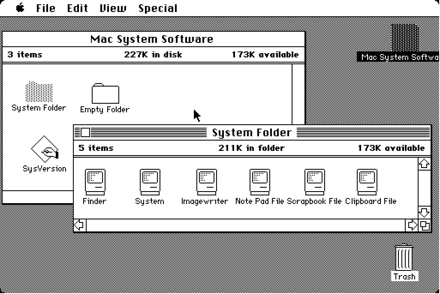
\includegraphics{xeorox}

\bf{Metaphors}
\begin{itemize}
    \item Desktop
    \item Paper Paradigm
    \item File System
    \item MailBoxes
    \item Timesharing
\end{itemize}
\subsection{Desktop}
The Desktop Metaphor is the one introduced by Alan Kay at Xerox Parc. It had all the items on your desk but within this magical computing device, such as, phone, calculator, word processor and even some rudimentary games.
 This was a metaphor that would stick to the masses of people because they know how to use all of those "desktop" items already now they can do it, at the time, arguably faster and more efficiently.
\subsection{Paper Paradigm}
The Paper Paradigm was following in the footsteps of the desktop metaphor.
Reaching to find familiar ground it seems like a natural follow up, and what a hit it was.  The best way of information transmission at scale is the text on paper method for thousands of years why change that now.
\subsection{File System}
This metaphor is rooted in filing cabinet.
We peer in them try to find our correct documents. We organize in much of the same ways. By Size, Name, Last Opened, so many algorithmic ways that we have thought of before computer to be translated into machine code.
\subsection{MailBoxes}
Mailbox is another tick for tac translation but with a little hint of superpowers.
With the ability to send large documents, video and text over the mail faster than we could've dreamed of before the computer age. It makes you wonder whether we should still be calling it mail or adhering to any of the metaphors, not for understanding sake but for accuracy's sake. The many magnitude of doing the counter part with its traditional analog counter part would be archaic compared to what we have now. But we keep these metaphor because they work and they have worked for a while.
\subsection{Time Sharing}
 Research Articles that will be used are in the research folder!
